\documentclass{article}

\usepackage{graphicx}
\usepackage{tikz}
\usepackage{tikzsymbols}
\usetikzlibrary{calc,patterns,shapes.geometric}
\pagestyle{empty}
\usepackage[margin=0pt]{geometry}
\geometry{papersize={14in,12in}}

\def\centerarc[#1](#2)(#3:#4:#5){\draw[#1] ($(#2)+({#5*cos(#3)},{#5*sin(#3)})$) arc (#3:#4:#5);}

\begin{document}
	\begin{figure}
		\centering
		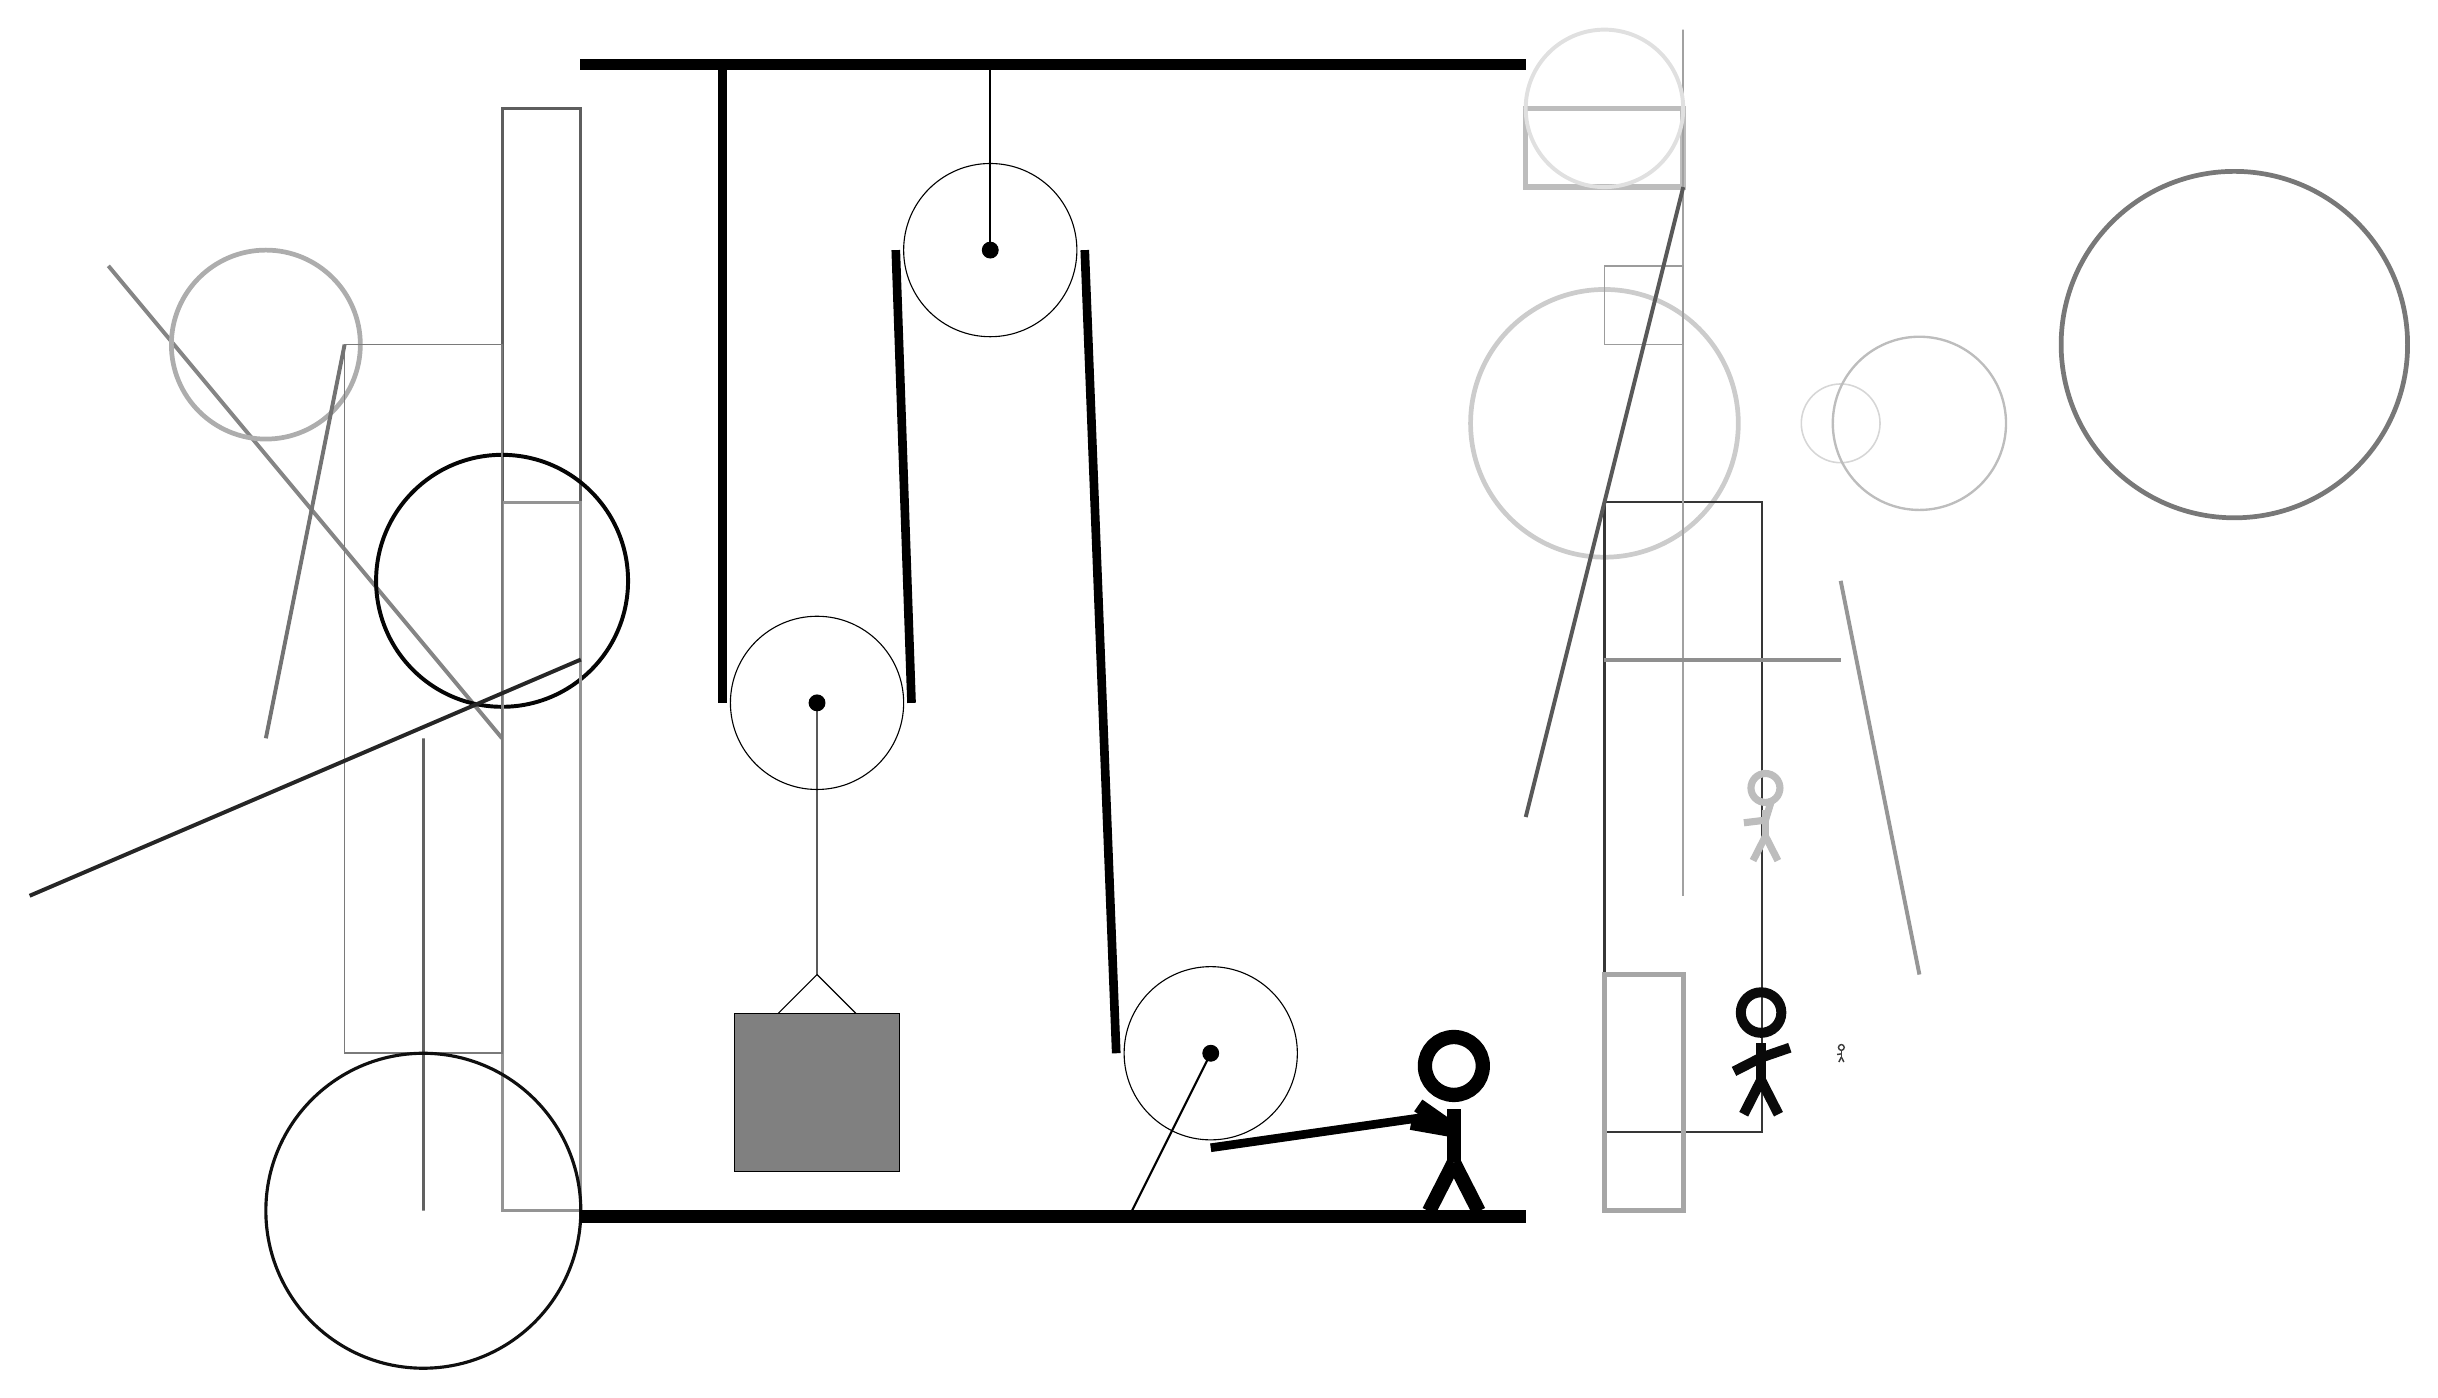
\begin{tikzpicture}
			%%%%% START %%%%%
			
			\draw[fill=black] (-2, 11.5) rectangle (10, 11.625);
			
			\draw (3.2, 9.2) circle (1.1);
			\draw[fill=black] (3.2, 9.2) circle (0.1);
			\draw[thick] (3.2, 9.2) -- (3.2, 11.5);
			
			\draw (6, -1) circle (1.1);
			\draw[fill=black] (6, -1) circle (0.1);
			\draw[thick] (6, -1) -- (5, -3);
			
			\draw (1, 3.45) circle (1.1);
			\draw[fill=black] (1, 3.45) circle (0.1);
			
			\draw (1, 3.45) -- (1, 0.0) -- (0.5, -0.5);
			\draw (1, 0.0) -- (1.5, -0.5);
			\draw[fill=black!50] (-0.05, -0.5) rectangle (2.05, -2.5);
			
			\draw[line width=1.1mm] (-0.2, 11.5) -- (-0.2, 3.45);
			\centerarc[line width=1.1mm](1, 3.45)(180:360:1.2000000000000002);
			\draw[line width=1.1mm](2.2, 3.45) -- (2.0, 9.2);
			\centerarc[line width=1.1mm](3.2, 9.2)(0:180:1.2000000000000002);
			\draw[line width=1.1mm](4.4, 9.2) -- (4.8, -1);
			\centerarc[line width=1.1mm](6, -1)(180:270:1.2000000000000002);
			\draw[line width=1.1mm](6, -2.2) -- (8.8, -1.8);
			
			\draw [line width=0.6mm, color=black!53](19, 8) circle (2.2);
			
			\draw [line width=0.2mm, color=black!16](14, 7) circle (0.5);
			\draw[line width=0.5mm, color=black!48](-3, 3) -- (-8, 9);
			\node[line width=0.7mm, color=black!76] at (14, -1) {\Strichmaxerl[1][8][90]};
			\draw[line width=0.4mm, color=black!62] (-4, -3) rectangle (-4, 3);
			
			\draw[line width=0.7mm, color=black!26] (12, 11) rectangle (10, 10);
			\draw[line width=0.4mm, color=black!63] (-2, 6) rectangle (-3, 11);
			\draw [line width=0.6mm, color=black!20](11, 7) circle (1.7);
			\draw[line width=0.3mm, color=black!79] (11, -2) rectangle (13, 6);
			\draw[line width=0.6mm, color=black!35] (11, -3) rectangle (12, 0);
			
			\draw [line width=0.5mm, color=black!98](-3, 5) circle (1.6);
			
			\draw[line width=0.5mm, color=black!41](14, 5) -- (15, 0);
			\draw[line width=0.4mm, color=black!42] (-2, -3) rectangle (-3, 6);
			
			\node[line width=0.2mm, color=black!26] at (13, 2) {\Strichmaxerl[5][7][73]};
			\draw[line width=0.3mm, color=black!37] (12, 1) rectangle (12, 12);
			\draw [line width=0.6mm, color=black!32](-6, 8) circle (1.2);
			
			\draw[line width=0.2mm, color=black!52] (-3, -1) rectangle (-5, 8);
			\draw[line width=0.2mm, color=black!39] (12, 9) rectangle (11, 8);
			\draw[line width=0.5mm, color=black!65](10, 2) -- (12, 10);
			\draw[line width=0.5mm, color=black!55](-6, 3) -- (-5, 8);
			\draw [line width=0.5mm, color=black!12](11, 11) circle (1.0);
			
			\draw [line width=0.3mm, color=black!26](15, 7) circle (1.1);
			\node[line width=0.3mm, color=black!96] at (13, -1) {\Strichmaxerl[7][27][19]};
			\draw [line width=0.4mm, color=black!94](-4, -3) circle (2.0);
			\draw[line width=0.5mm, color=black!44](14, 4) -- (11, 4);
			
			\draw[line width=0.5mm, color=black!85](-2, 4) -- (-9, 1);
			
			\node at (9, -1.9) {\Strichmaxerl[10][-35][170]};
			
			\draw[fill=black] (-2, -3) rectangle (10, -3.15);
			
			%%%%% END %%%%%
		\end{tikzpicture}
	\end{figure}	
\end{document}